\documentclass[12pt, a4paper, twoside]{article}

%% Preamble
\usepackage{pdfpages}           % Para incluir PDFs
\usepackage{graphicx}           % Para gráficos
\usepackage{subfiles}           % Para manejar subarchivos
\usepackage{hyperref}           % Para enlaces
\usepackage{listings}           % Para código fuente (ajusta lenguaje)
\usepackage{verbatim}
\usepackage[backend=bibtex,style=numeric]{biblatex} % Para citas numéricas
\addbibresource{references.bib} % Cargar archivo .bib
\usepackage{url}


\usepackage{geometry}           % Para ajustar márgenes

% Ajustes de márgenes
\geometry{
	left=3cm,       % Margen izquierdo
	right=3cm,      % Margen derecho
	top=2.5cm,      % Margen superior
	bottom=2.5cm,   % Margen inferior
	headheight=15pt, % Altura del encabezado
	twoside          % Para documentos a dos caras
}


\graphicspath{{images/}{../images/}} % Ruta para imágenes

\begin{document}
	
	%% Cover
	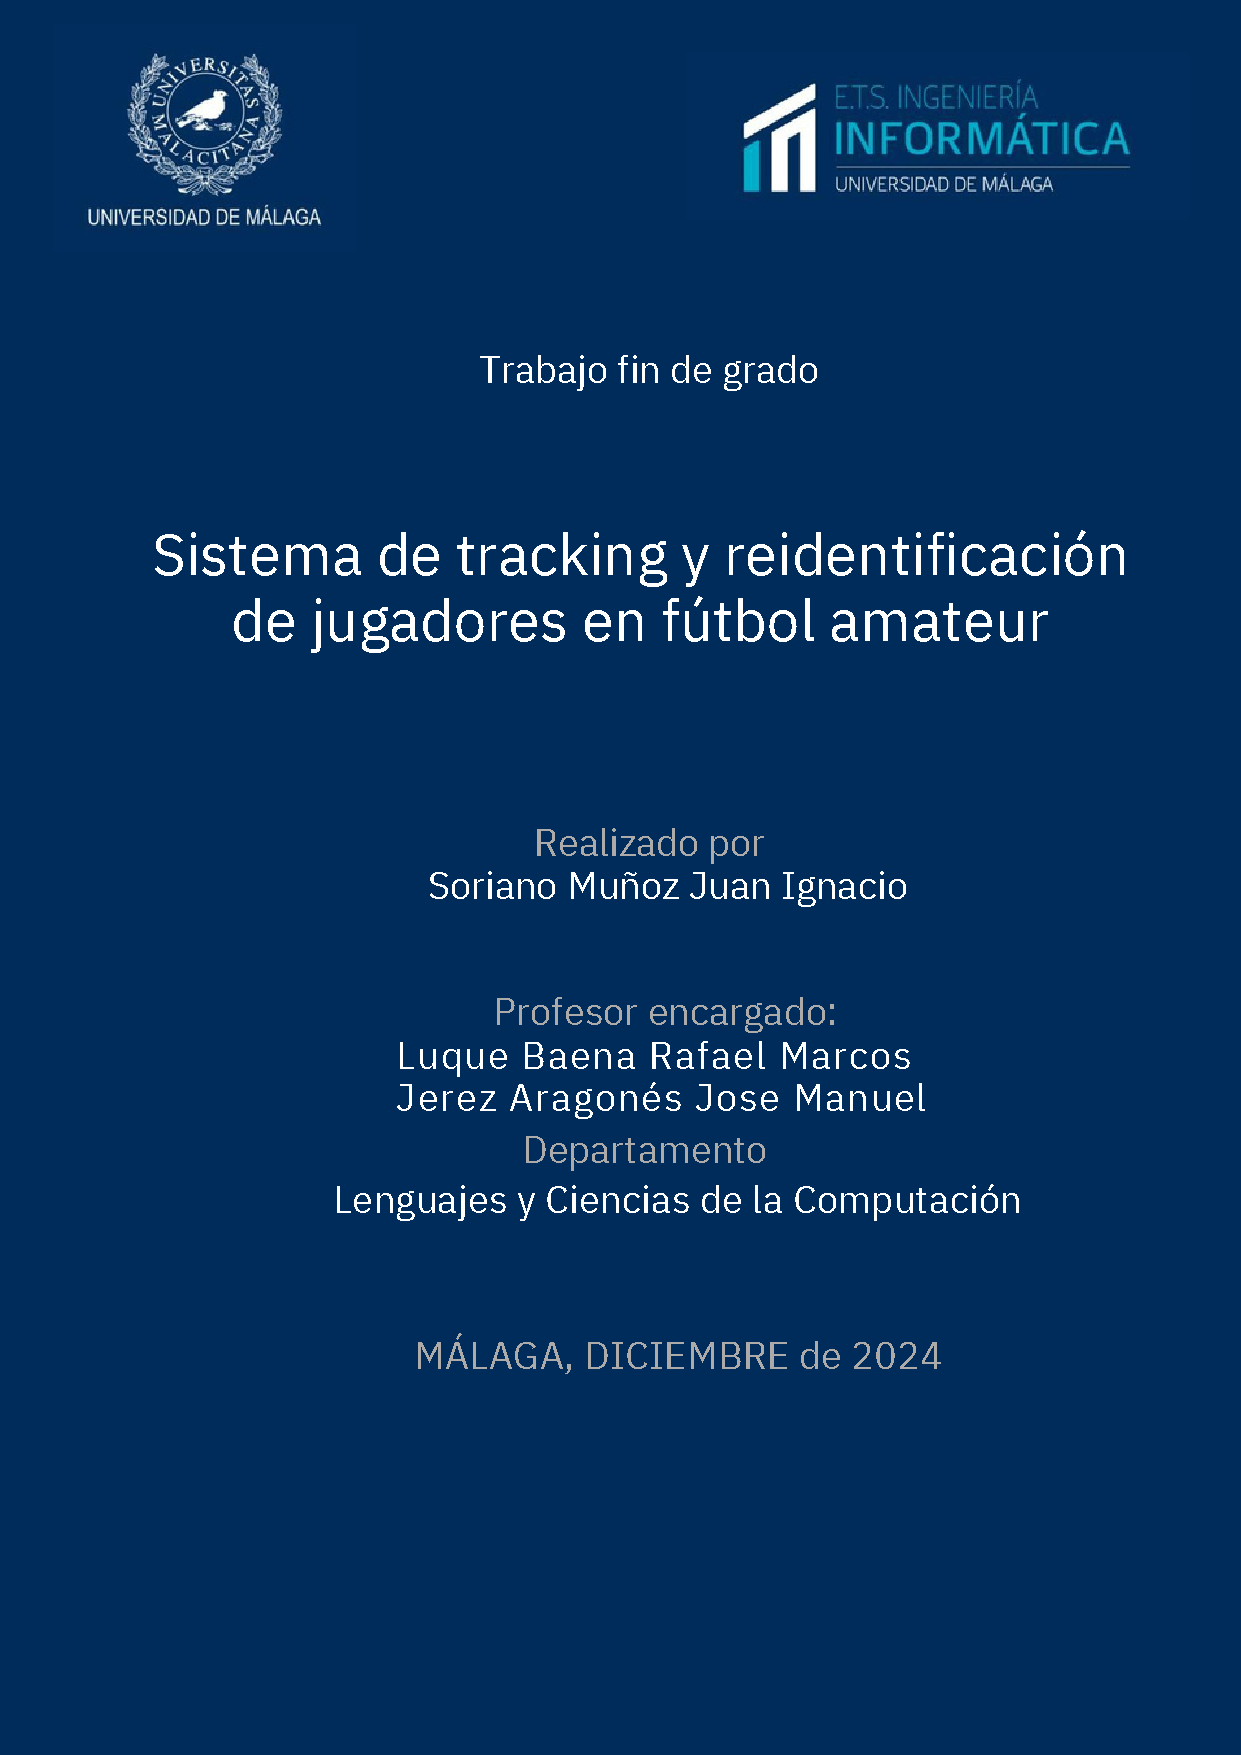
\includepdf[noautoscale=true, width=\paperwidth]{cover.pdf}
	
	%% Title
	\clearpage
	\setcounter{page}{1}
	
\includepdf[noautoscale=true, width=\paperwidth]{title.pdf}
	
	%%%%%%%%%%%%%%%%%%%%%%%%%%%%%%%%%%%%%%%%%%%%%%%%%%%%%%%%%%%%%%%%%%%%%%%%%%%
	
	% Índice automático
	\tableofcontents
	\newpage
	
	% Sections
	
		% Sections
	\section{Introducción}
	
	\section{Diario de avances}
	
	\subsection{Semana 3-16 de marzo)}
	
	Por ahora lo que llevamos es un dataset hecho en roboflow con un partido de España contra Suiza. Realizamos capturas y dividimos el conjunto en training, validation y test.
	
	Entrené el modelo de YOLO con este dataset revisado y el modelo no supo detectar bien el balón debido a la poca cantidad de imágenes donde se pueda ver bien la bola. El árbitro y los jugadores fueron bien detectados.
	
	Se replanteó el objetivo del TFG. Se focalizará en la reidentificación de jugadores cuando salen fuera de plano y en el desarrollo de una aplicación que permita al usuario decidir si cuando se produce un cambio de identificador, mantenerlo o cambiarlo, creando un dataset revisado.
	
	\subsection{Semana 17-31 de marzo \cite{sun2024gta}}
	
	A la hora de medir resultados como estas gráficas:
	
	\begin{figure}[h]
		\centering
		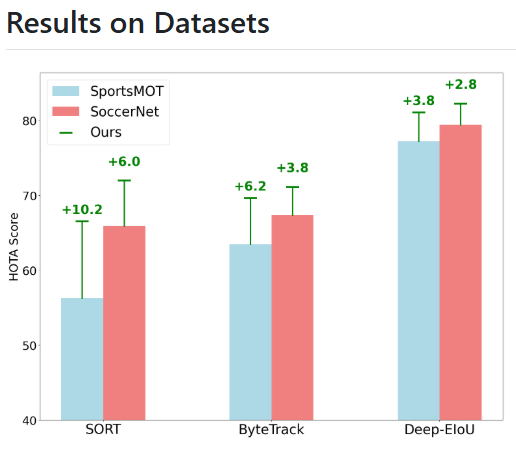
\includegraphics[width=0.8\textwidth]{image/metricasBeta}
		\caption{\textbf{Métricas gta\_link}}
		\label{fig:metricasBeta}
	\end{figure}
	
	Nos centraremos en la medida de los ID's intentando minimizarlos, lo máximo posible, ya que la métrica significa número de ids generados.
	
	\begin{figure}[h]
		\centering
		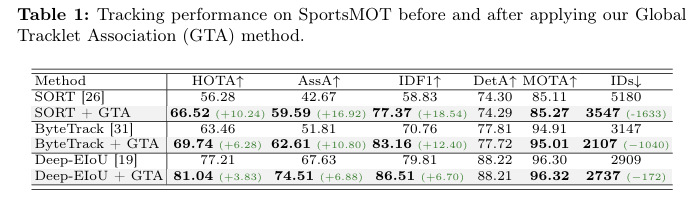
\includegraphics[width=0.8\textwidth]{image/Centrarse}
		\caption{\textbf{Objetivo}}
		\label{fig:Centrarse}
	\end{figure}
	
	Me he puesto a mirar lo que hace exactamente el código del repositorio de gta-link. Y en resumidas cuentas necesitamos un dataset con una pred, ya realizada, como es el caso de SoccerNet. Podemos descargar el dataset con el tracking realizado en los archivos .txt que se encuentran dentro de cada clip.\vspace{0.5cm}
	
	He utilizado las siguientes líneas de comando para realizar la descarga del dataset.
	
	\begin{verbatim}
		from SoccerNet.Downloader import SoccerNetDownloader
		mySoccerNetDownloader = SoccerNetDownloader(LocalDirectory="path/to/SoccerNet")
		mySoccerNetDownloader.downloadDataTask(task="tracking",
		 split=["train","test","challenge"])
	\end{verbatim}
	
	Posteriormente hice unos ajustes en el código para que cogiera los archivos \texttt{gt.txt} para que se tomara como referencia \textbf{--pred\_dir {tracking results directory}}, ya que estos son archivos \textbf{MOT}, que guardan información sobre los \textbf{bounding box} de cada objeto de cada frame, conteniendo información sobre \textbf{frame}, \textbf{id}, \textbf{bb\_left}, \textbf{bb\_top}, \textbf{bb\_width}, \textbf{bb\_height}, \textbf{conf}, \textbf{x}, \textbf{y}, \textbf{z}, en este orden.
	
	Estos son esenciales para que se pueda ejecutar el archivo \texttt{generate\_tracklets.py} para generar los \textbf{tracklets}.
	
	Un \textbf{tracklet} se genera al seguir a un objeto desde su detección en un fotograma hasta el siguiente. En este proceso, el código asocia las detecciones de objetos de cada fotograma con un identificador único (\textbf{ID}) para cada objeto, y los agrupa en una \textbf{"trayectoria"} que sigue ese objeto a lo largo del tiempo.
	
	En el código:
	
	\begin{itemize}
		\item \textbf{Extracción de características:} El código utiliza un modelo de reidentificación de personas (\texttt{FeatureExtractor}) para extraer características visuales de cada objeto detectado en los fotogramas. Esto es útil para seguir objetos entre fotogramas, incluso cuando se producen cambios de apariencia debido a variaciones en la vista o el movimiento.
		\item \textbf{Cálculo de tracklets:} Para cada fotograma, el código agrupa las detecciones de objetos utilizando el identificador único (\texttt{track\_id}). Si un objeto se detecta en un fotograma y luego aparece en otro, se agrega a un tracklet, que es una colección de todas las detecciones del mismo objeto a lo largo de varios fotogramas. Además, se guarda información como el puntaje de la detección y las características extraídas del modelo de reidentificación.
		\item \textbf{Salvado de tracklets:} Al final de cada secuencia de video o serie de fotogramas, los tracklets generados se guardan en un archivo \texttt{pickle} para su posterior uso, permitiendo analizar y trabajar con las trayectorias de los objetos en el futuro.
	\end{itemize}
	
	El programa \texttt{generate\_tracklets.py}, lo que hará será generar unos ficheros \texttt{.pkl} que guardan los datos de las trayectorias de los objetos detectados a lo largo del tiempo. Esto incluye, por ejemplo, las \textbf{detecciones de objetos en cada fotograma}, las \textbf{características extraídas por el modelo de reidentificación}, y los \textbf{identificadores únicos (ID)} asignados a cada objeto (en formato binario).
	
	Una vez que se tenga esos ficheros se realiza una \textbf{refinación de los tracklets} para evitar que se cambien los \textbf{ids con frecuencia}. Mejora los \textbf{tracklets} (trayectorias de objetos) generados por un \textbf{tracker en tareas de seguimiento de múltiples objetos (MOT)}. Utiliza dos componentes principales: el \textbf{Tracklet Splitter}, que divide \textbf{tracklets impuros} (con múltiples identidades) en subtracklets más precisos mediante \textbf{clustering (DBSCAN)}, y el \textbf{Tracklet Connector}, que fusiona \textbf{tracklets fragmentados} que pertenecen al mismo objeto basándose en \textbf{similitudes visuales y restricciones espaciales}. Los resultados refinados se guardan en archivos \texttt{.txt} en formato \textbf{MOT}, listos para su evaluación, visualización o análisis posterior. Este proceso optimiza la \textbf{precisión del seguimiento}, corrigiendo errores como \textbf{cambios de identidad} y \textbf{fragmentaciones}.\vspace{0.5cm}
	
	
	Ahora que tenemos un dataset etiquetado, tendremos que:
	
	\begin{itemize}
		\item \textbf{Encontrar una combinación de hiperparámetros óptima: } Con el objetivo de que el cambio de ids sea el mínimo posible.
		\item \textbf{Desarrollar una aplicación: } Con el objetivo de que avise al usuario sobre los cambios de id en los frames y confirme si está bien cambiado o debería conservarse el anterior.
	\end{itemize}
	
	\subsection{Semana 31-6 de abril)}
	
	En estas semanas hemos estado invirtiendo tiempo en las siguientes cosas. En un principio lo que teníamos era un dataset preparado con los ficheros ground truth fruto de un tracker usado (como DeepEIoU). Pero dado un vídeo, no podíamos aplicar los programas de gta-link, por lo que teníamos que conseguir los ficheros MOT de alguna manera. 
	
	Había dos opciones. La primera aplicar un tracker y la segunda aplicar un modelo de YOLO.
	
	Para la primera opción busqué en varios repositorios, que trataran con trackers, principalmente DeepEIoU, que es el tracker con el mejor rendimiento según las estadísticas de paperscode \cite{sportsmot_paperswithcode}.
	
	\begin{figure}[h]
		\centering
		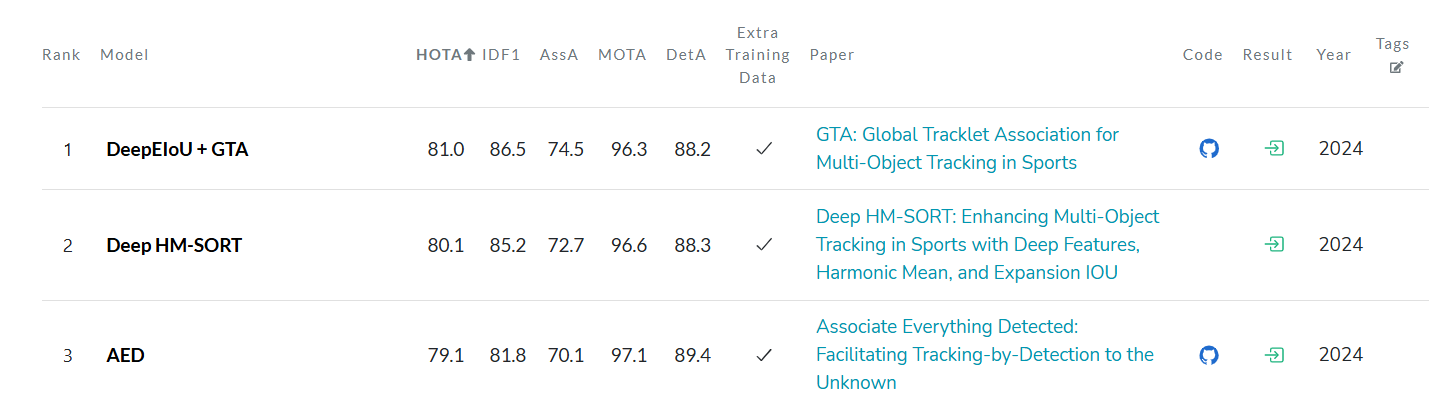
\includegraphics[width=0.8\textwidth]{image/deepEIoU}
		\caption{\textbf{Métricas DeepEIoU}}
		\label{fig:deepEIoU}
	\end{figure} 
	
	Tras encontrar un repositorio que trataba en específico con este \cite{huang2024iterative}. Tuve que modificar código para que utilizara cpu, ya que estaba configurado para gpu de nvidia. Los paquetes no se me instalaban correctamente. Los inputs que utilizaba para los programas eran ficheros tipo .npy.
	
	Dado que me estaba dando muchos problemas, después de dos días decidí que la mejor solución era utilizar un modelo de YOLO. Empecé utilizando un modelo de YOLO estandar capaz de detectar personas. El inconveniente de esto es que el video, estaba grabado desde un ángulo muy bajo, por lo que el modelo detectara las personas de las gradas y esto, a la larga, es un problema. 
	
	Entonces para resolver esto había dos opciones. La primera era realizar una segmentación del campo y la segunda entrenar un modelo de YOLO específico para jugadores. La segmentación del campo es demasiado costosa, porque no hay nada automatizado y sería segmentar infinidad de frames. Además de que es específica para un partido de fútbol en un ángulo en específico.Por lo tanto, la mejor opción para mi gusto es entrenar un modelo de YOLO con un dataset, por ahora, específico del partido de balonmano que me proporcionó mi tutor Jose Manuel Jerez. El dataset lo hice creando un programa utilizando las librerias de opencv (cv2) que extraía frames cada 20 segundos que transcurría de vídeo. Los 20 segundos previenen levemente más overfitting del que ocurre por tener frames del mismo partido. 
	
	Esta opción me permite etiquetar poco, ya que Roboflow tiene una herramienta de etiquetado automático una vez se han etiquetado unas cuantas imágenes, por lo que simplemente tuve que corregir aquellas imágenes con un mal etiquetado.
	
	Tras tener el dataset etiquetado le añadí algunas augmentations. 
	
	A la hora de entrenar el modelo lo hice con 25 epochs. Tardó hora y media en entrenarse.
	
	Apliqué los programas del repositorio de gta-link y los resultados del trackeo son muy buenos, pero la ReID no tiene nada que ver con los resultados tan consistentes del dataset de SoccerNet debido a que la grabación no es profesional.
	
	Aun así tras 23 intentos observe que los parámetros que daban mejores resultados eran los siguientes: --use\_split --min\_len 100 --eps 0.8 --min\_samples 10 --max\_k 4 --use\_connect --spatial\_factor 1.0 --merge\_dist\_thres 0.7   
	
	Recientemente le he añadido frames del partido de fútbol 7 al dataset de roboflow. Y he creado un nuevo modelo de YOLO entrenado exclusivamente con ese dataset.
	
	Los objetivos para la próxima semana:
	
	\begin{itemize}
		\item \textbf{Buscar como aplicar un tracker:} Después de aplicar un trackeo con YOLO, sería necesario aplicar DeepEIoU. Investigar si aplicar un doble gta-link puede funcionar para refinar los tracklets todavía más.
		\item \textbf{Seguir desarrollando la aplicación: } Con el objetivo de que avise al usuario sobre los cambios de id en los frames y confirme si está bien cambiado o debería conservarse el anterior. Ya tengo un programa prueba\_revision\_ReID.py, que funciona como prototipo, pero falta desarrollarlo mucho.
	\end{itemize}
	
	
	%%%%%%%%%%%%%%%%%%%%%%%%%%%%%%%%%%%%%%%%%%%%%%%%%%%%%%%%%%%%%%%%%%%%%%%%%%%
	\printbibliography
	
	
	%% Back Cover
	
\includepdf[noautoscale=true, width=\paperwidth]{backcover.pdf}
	
\end{document}